\documentclass[12pt, border=12pt]{standalone}
\usepackage[T1]{fontenc}
\usepackage{tikz}
\usepackage{helvet}
\renewcommand{\familydefault}{\sfdefault}
\usetikzlibrary{shapes.geometric, arrows.meta, positioning, fit, backgrounds, calc, shadows}

\begin{document}
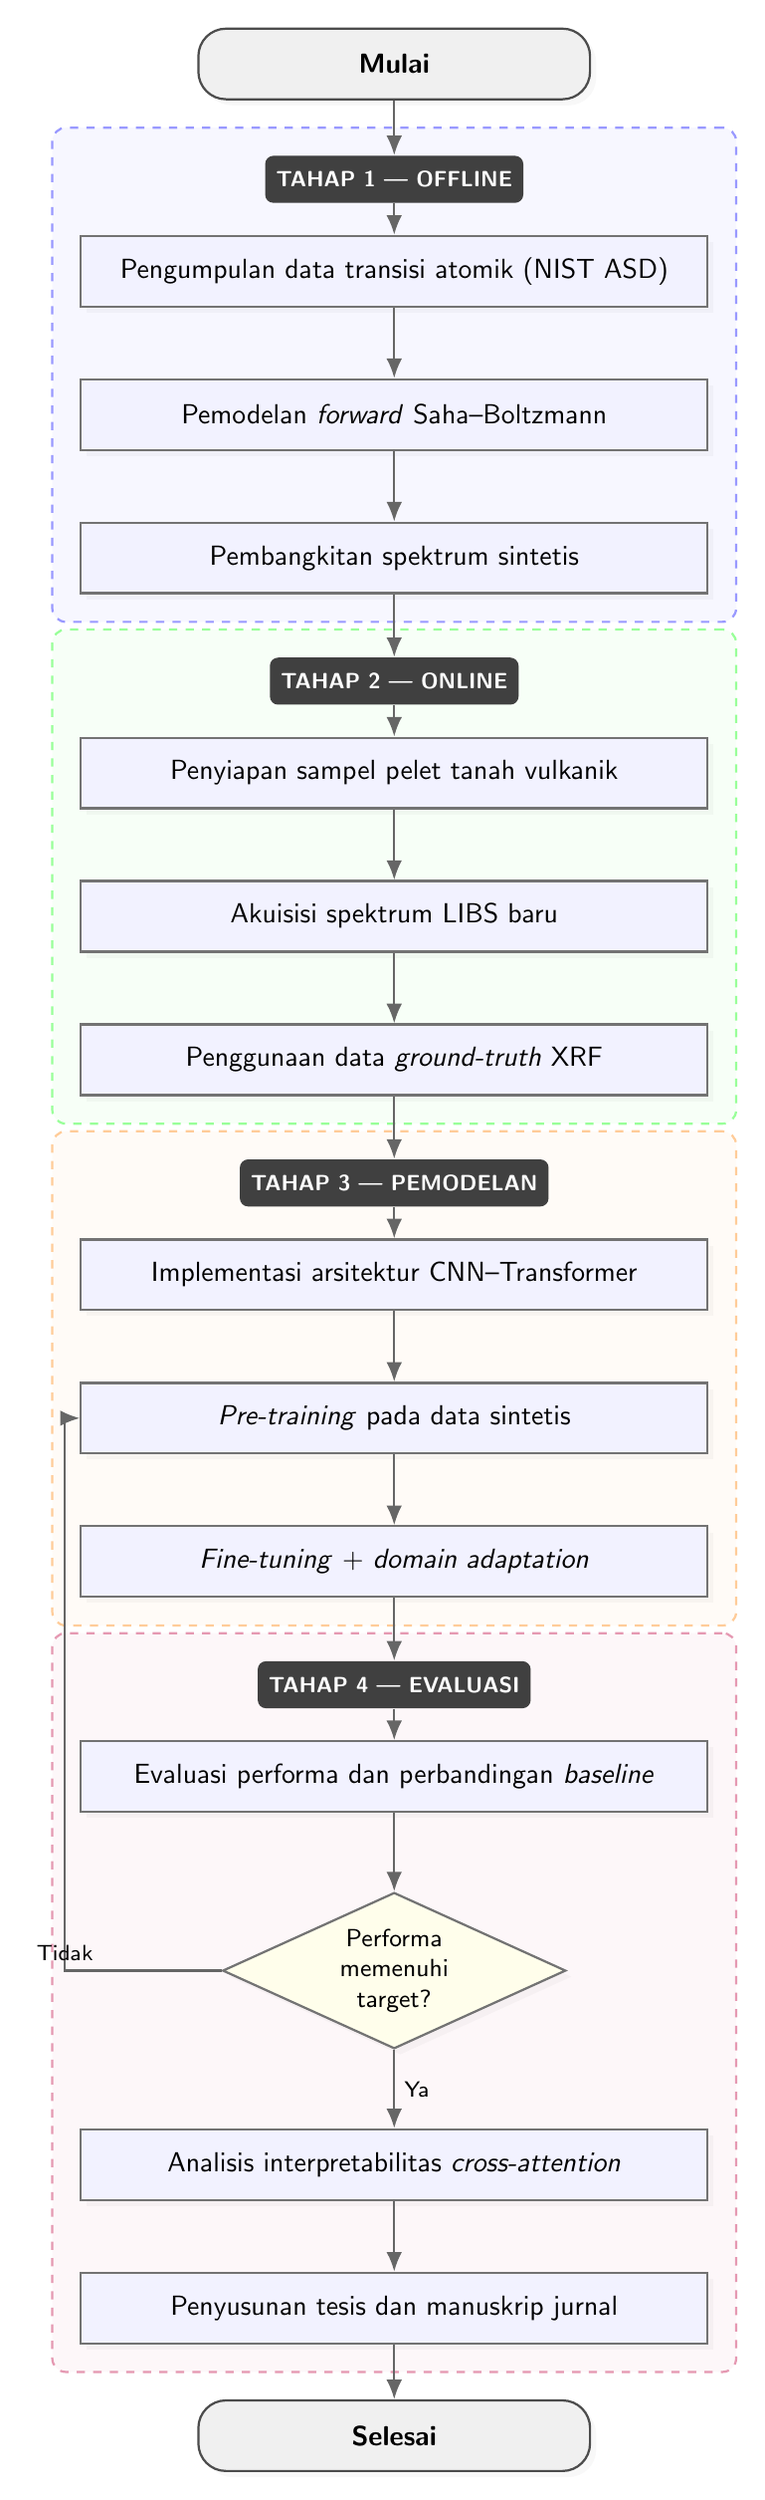
\begin{tikzpicture}[
    node distance = 0.9cm,
    % --- Node styles ---
    startstop/.style = {rectangle, rounded corners=10pt, draw=black!70, thick,
        fill=gray!12, minimum width=5cm, minimum height=0.9cm, align=center,
        font=\normalsize\bfseries, drop shadow={opacity=0.06}},
    process/.style = {rectangle, draw=black!55, thick, fill=blue!5,
        minimum width=8cm, minimum height=0.9cm, align=center,
        font=\normalsize, inner sep=7pt, drop shadow={opacity=0.05}},
    decision/.style = {diamond, draw=black!55, thick, fill=yellow!8,
        minimum width=2.5cm, aspect=2.2, align=center,
        font=\small, inner sep=3pt, drop shadow={opacity=0.05}},
    phase/.style = {rectangle, rounded corners=3pt, draw=none,
        fill=black!75, text=white, font=\footnotesize\bfseries,
        minimum height=0.6cm, inner sep=4pt},
    % --- Arrow style ---
    arrow/.style = {thick, -{Latex[length=2.5mm, width=2mm]}, draw=black!60},
    % --- Group box ---
    groupbox/.style = {rectangle, draw=#1!40, thick, dashed, rounded corners=5pt,
        fill=#1!3, inner sep=10pt}
]

% ==================== START ====================
\node[startstop] (mulai) {Mulai};

% ==================== TAHAP 1 ====================
\node[phase, below=0.7cm of mulai] (fase1) {TAHAP 1 --- OFFLINE};

\node[process, below=0.4cm of fase1] (p1) {Pengumpulan data transisi atomik (NIST ASD)};

\node[process, below=of p1] (p2) {Pemodelan \textit{forward} Saha--Boltzmann};

\node[process, below=of p2] (p3) {Pembangkitan spektrum sintetis};

% ==================== TAHAP 2 ====================
\node[phase, below=0.8cm of p3] (fase2) {TAHAP 2 --- ONLINE};

\node[process, below=0.4cm of fase2] (p4) {Penyiapan sampel pelet tanah vulkanik};

\node[process, below=of p4] (p5) {Akuisisi spektrum LIBS baru};

\node[process, below=of p5] (p5b) {Penggunaan data \textit{ground-truth} XRF};

% ==================== TAHAP 3 ====================
\node[phase, below=0.8cm of p5b] (fase3) {TAHAP 3 --- PEMODELAN};

\node[process, below=0.4cm of fase3] (p6) {Implementasi arsitektur CNN--Transformer};

\node[process, below=of p6] (p7) {\textit{Pre-training} pada data sintetis};

\node[process, below=of p7] (p8) {\textit{Fine-tuning} + \textit{domain adaptation}};

% ==================== TAHAP 4 ====================
\node[phase, below=0.8cm of p8] (fase4) {TAHAP 4 --- EVALUASI};

\node[process, below=0.4cm of fase4] (p9) {Evaluasi performa dan perbandingan \textit{baseline}};

\node[decision, below=1cm of p9] (dec1) {Performa\\memenuhi\\target?};

\node[process, below=1cm of dec1] (p10) {Analisis interpretabilitas \textit{cross-attention}};

\node[process, below=of p10] (p11) {Penyusunan tesis dan manuskrip jurnal};

\node[startstop, below=0.7cm of p11] (selesai) {Selesai};

% ==================== ARROWS ====================
\draw[arrow] (mulai) -- (fase1);
\draw[arrow] (fase1) -- (p1);
\draw[arrow] (p1) -- (p2);
\draw[arrow] (p2) -- (p3);
\draw[arrow] (p3) -- (fase2);
\draw[arrow] (fase2) -- (p4);
\draw[arrow] (p4) -- (p5);
\draw[arrow] (p5) -- (p5b);
\draw[arrow] (p5b) -- (fase3);
\draw[arrow] (fase3) -- (p6);
\draw[arrow] (p6) -- (p7);
\draw[arrow] (p7) -- (p8);
\draw[arrow] (p8) -- (fase4);
\draw[arrow] (fase4) -- (p9);
\draw[arrow] (p9) -- (dec1);
\draw[arrow] (dec1) -- node[right, font=\footnotesize] {Ya} (p10);
\draw[arrow] (p10) -- (p11);
\draw[arrow] (p11) -- (selesai);

% Decision "Tidak" loop back
\draw[arrow] (dec1.west) -- ++(-2,0) node[above, font=\footnotesize] {Tidak} |- (p7.west);

% ==================== GROUP BOXES ====================
\begin{scope}[on background layer]
    \node[groupbox=blue, fit=(fase1) (p1) (p2) (p3)] {};
    \node[groupbox=green, fit=(fase2) (p4) (p5) (p5b)] {};
    \node[groupbox=orange, fit=(fase3) (p6) (p7) (p8)] {};
    \node[groupbox=purple, fit=(fase4) (p9) (dec1) (p10) (p11)] {};
\end{scope}

\end{tikzpicture}
\end{document}
